\documentclass{article}

\usepackage[most]{tcolorbox}
\usepackage{physics}
\usepackage{graphicx}
\usepackage{float}
\usepackage{amsmath}
\usepackage{amssymb}


\usepackage[utf8]{inputenc}
\usepackage[a4paper, margin=1in]{geometry} % Controla los márgenes
\usepackage{titling}

\title{Tarea 2}
\author{Manuel Garcia.}
\date{\today}

\renewcommand{\maketitlehooka}{%
  \centering
  \vspace*{0.05cm} % Espacio vertical antes del título
}

\renewcommand{\maketitlehookd}{%
  \vspace*{2cm} % Espacio vertical después de la fecha
}

\newcommand{\caja}[3]{%
  \begin{tcolorbox}[colback=#1!5!white,colframe=#1!25!black,title=#2]
    #3
  \end{tcolorbox}%
}

\begin{document}
\maketitle

\section{Formas}

\textbf{a) } 
\begin{itemize}
  \item De la definicion $ d\omega = \partial_i \omega dx_i $, entonces: 
    \begin{gather*}
      d(d\omega) = \partial_i(\partial_j\omega)dx_i \wedge dx_j 
    \end{gather*}
    Los terminos con i=j se simplifican a 0 ya que $ dx_i\wedge dx_j= 0 $ y nos queda:
    \begin{gather*}
      d(d\omega) =  \partial_i(\partial_j\omega)dx_i \wedge dx_j - \partial_j(\partial_i\omega)dx_j \wedge dx_i \qquad \text{Para }i\neq j
    \end{gather*}
    Como $ dx_i\wedge dx_j = - dx_j \wedge dx_i  $ 
    \begin{gather*}
      d(d\omega) = 0 
    \end{gather*}

  \item 
  \begin{gather}
    d(\omega \wedge \eta) = \partial_i(\omega\wedge \eta) dx_i \qquad \qquad \omega \wedge \eta = \omega_I \eta_J dx^I\wedge dx^J
  \end{gather}
  Entonces: 
  \begin{align*}
    d(\omega \wedge \eta) &=  \partial_i(\omega_I \eta_J) dx_i \wedge dx^I \wedge dx^J\\
             &= (\partial_i\omega_I) \eta_J dx_i \wedge dx^I \wedge dx^J + \omega_I (\partial_i \eta_J) dx_i \wedge dx^I \wedge dx^J
  \end{align*}
  Usando que $ dx_i \wedge dx^I = (-1)^p dx^I\wedge dx_i  $
  \begin{gather*}
    d(\omega \wedge \eta) = (\partial_i\omega_I) \eta_J dx_i \wedge dx^I \wedge dx^J + \omega_I (\partial_i \eta_J) (-1)^p dx^I\wedge dx_i \wedge dx^J
  \end{gather*}
  Usando que $ d\omega \wedge \eta = (\partial_i\omega_I) \eta_J dx_i\wedge dx^I \wedge dx^J $ y que $ \omega \wedge d\eta = \omega_I (\partial_i \eta_J) dx^I \wedge dx_i \wedge dx^J $, tenemos:
  \begin{gather*}
    d(\omega\wedge\eta) = d\omega \wedge \eta + (-1)^p(\omega \wedge d\eta) 
  \end{gather*}

  \item 

  \item 
    Tenemos que $ d\omega=\partial_i \omega dx^i $, entonces: 
    \begin{gather*}
       V\lrcorner(d\omega) = \partial_i\omega_I dx_i\wedge dx^I = - \displaystyle\sum_{i=1 }^{}\partial_i\omega_I dx_i \wedge dx^I
    \end{gather*}
    Tenemos que $ V \lrcorner \omega = \omega_I dx^I $:
    \begin{gather*}
       d(V \lrcorner \omega) = \displaystyle\sum_{i=0 }^{} \partial_i \omega_I dx_i \wedge dx^I
    \end{gather*}
    Entonces: 
    \begin{align*}
      V\lrcorner(d\omega) + d(V\lrcorner\omega) &= - \displaystyle\sum_{i=1 }^{}\partial_i\omega_I dx_i \wedge dx^I +  \displaystyle\sum_{i=0 }^{} \partial_i \omega_I dx_i \wedge dx^I \\&= - \displaystyle\sum_{i=1 }^{}\partial_i\omega_I dx_i \wedge dx^I + \partial_0\omega dx^0\wedge dx^I +  \displaystyle\sum_{i=1 }^{} \partial_i \omega_I dx_i \wedge dx^I \\
                      &= \partial_0\omega dx^0\wedge dx^I = \mathcal{L}_V \omega 
    \end{align*}

  \item 
    \begin{align*}
      \mathcal L _V (d\omega) &= \partial_0 \partial_i \omega_I dx_0 \wedge dx^I \wedge dx_i  \\
      d(\mathcal L_V \omega) &= \partial_i\partial_0 \omega_I dx_0\wedge dx^I \wedge dx_i \\
                             &= \partial_0 \partial_i \omega_I dx_0 \wedge dx^I \wedge dx_i = \mathcal L_V(d\omega)
    \end{align*}

\end{itemize}


\textbf{b) }
\begin{gather*}
  \chi = x \partial_y - y \partial_x + z \partial_z \\
  \omega = x^2 z dx \wedge dy + y^2 dy\wedge dz
\end{gather*}
\begin{itemize}
  \item 
    \begin{align*}
      d\omega = d(x^2z dx \wedge dx) + d(y ^2 dy \wedge dz) &= (dx ^2 z) \wedge dx \wedge dy + (dy^2) \wedge dy \wedge dz \\
                &= 2zx \underset{=0 }{dx\wedge dx }\wedge dy + x^2 dz\wedge dx \wedge dy + 2y \underset{=0 }{dy\wedge dy }\wedge dz \\
                &= x^2 dx\wedge dy \wedge dz 
    \end{align*}
  \item 
    \begin{align*}
      \mathcal L_\chi \omega &= X^\lambda \partial_\lambda \omega + \omega \partial_\nu X^\lambda + \omega \partial_\mu X^\rho\\
                             &= (x^2 - 2xy)zdx\wedge dy + y^2 dx \wedge dz + (2xy + y^2) dy\wedge dz 
    \end{align*}
  \item 
    \begin{align*}
      X\lrcorner \omega &= X \lrcorner (x^2 z dx \wedge dy + y^2 dy\wedge dz) \\
           &= X \lrcorner x^2 z dx \wedge dy + X\lrcorner y^2 dy \wedge dz \\
           &= x^2z(-ydy-xdx)+y^2(xdz-zdy)\\
           &= -x^3zdx - (x^2 + y )zydy + xy^2 dz 
    \end{align*}

  \item 
\end{itemize}




\section{Lie Bracket}
\begin{gather*}
  [X,Y] \equiv X(Y(f)) - Y(X(f)) 
\end{gather*}

\begin{itemize}
  \item 
    \begin{align*}
      XY(fg) = X(Y(fg)) &= X(Y(f)g + fY(g))
                        &= X(Y(f))g + Y(f)X(g)+X(f)Y(g) + fX(Y(g))
    \end{align*}
    No cumple la regla de leibniz 
    \begin{align*}
      XY(fg)\neq XY(f)g + fXY(g)
    \end{align*}
  \item 
    \begin{align*}
      [X,Y] (fg) &= X(Y(f)g + fY(g)) - Y(X(f)g + fX(g))\\
      &= XY(f)g + Y(f)X(g) + X(f)Y(g) + f XY(g) - YX(f)g - X(f) Y(g) - Y(f)X(g) - fYX(g) \\
      &= (XY(f) - YX(f))g + f(XY(g) - YX(g)) \\
      &= [X,Y] (f) g + f[X,Y](g)
    \end{align*}
    Satisface la regla de Leibniz 
  \item Tenemos que $ X = X^\mu \partial_\mu  $  
    \begin{align*}
      [X,Y] &= X^\mu \partial_\mu (Y^\mu \partial_nu ) - Y^\mu \partial_\mu (X^\nu \partial_nu) \\
      &= (X^\mu \partial_\mu Y^\nu - Y^\mu \partial_\mu X^\nu) \partial_\nu
    \end{align*}
    Por lo tanto 
    \begin{align*}
      [X,Y]^\mu = X^\lambda \partial_\lambda Y^\mu - Y^\lambda \partial_\lambda X^\mu 
    \end{align*}
    Y tambien :
    \begin{align*}
      [Y,X]^\mu = Y^\lambda \partial_\lambda X^\mu - X^\lambda \partial_\lambda Y^\mu = - (X^\lambda \partial_\lambda Y^\mu - Y^\lambda \partial_\lambda X^\mu) = - [X,Y]^\mu
    \end{align*}

  \item 
    \begin{gather*}
      [X,[Y,Z]] +  [Y,[Z,X]] + [Z,[X,Y]] \\= XYZ - XZY - YZX +ZYX + YZX -ZXY -ZXY +XZY + ZXY -ZYX -XYZ +YXZ \\
      =0
    \end{gather*}
\end{itemize}


\section{Diagramas de ESpacio-Tiempo  }
\textbf{a) }
\begin{figure}[h!]
    \centering
    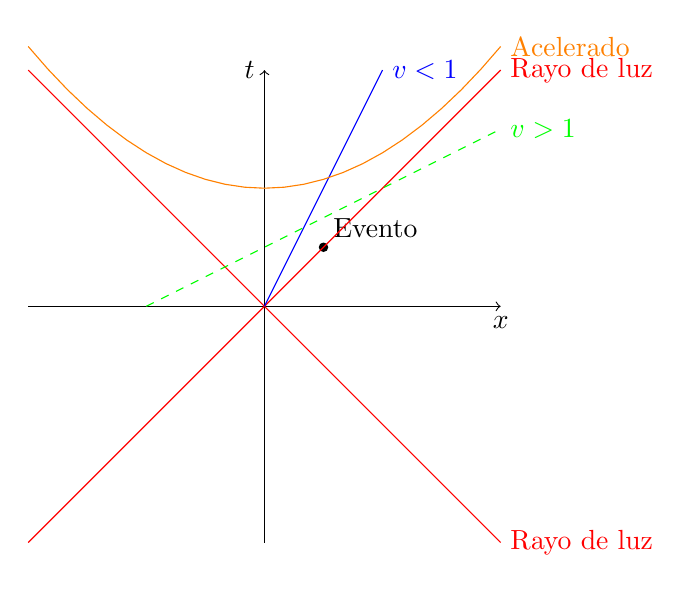
\begin{tikzpicture}[scale=1.5]
        % Axis
        \draw[->] (-2,0) -- (2,0) node[anchor=north]{$x$};
        \draw[->] (0,-2) -- (0,2) node[anchor=east]{$t$};
        
        % Event
        \filldraw (0.5,0.5) circle (1pt) node[anchor=south west]{Evento};

        % Light ray
        \draw[red] (-2,-2) -- (2,2) node[anchor=west]{Rayo de luz};
        \draw[red] (-2,2) -- (2,-2) node[anchor=west]{Rayo de luz};

        % World line v < 1
        \draw[blue] (0,0) -- (1,2) node[anchor=west]{$v < 1$};

        % World line v > 1
        \draw[dashed,green] (-1,0) -- (2,1.5) node[anchor=west]{$v > 1$};

        % Accelerated object
        \draw[orange,domain=-2:2] plot (\x, {0.3*\x*\x+1}) node[anchor=west]{Acelerado};
    \end{tikzpicture}
\end{figure}

\textbf{b) }
\begin{figure}[H]
    \centering
    \begin{tikzpicture}[scale=1.5]
        % Axis for O
        \draw[->] (-2,0) -- (2,0) node[anchor=north]{$x$};
        \draw[->] (0,-2) -- (0,2) node[anchor=east]{$t$};

        % World line of O'
        \draw[blue] (0,-2) -- (1,2) node[anchor=west]{$O'$};
        
        % Axis for O'
        \draw[dashed,red] (1,-2) -- (-1,2) node[anchor=west]{$x'$};
        \draw[dashed,red] (-1,-2) -- (1,2) node[anchor=east]{$t'$};
    \end{tikzpicture}
\end{figure}


\textbf{c) }
\begin{figure}[H]
    \centering
\begin{tikzpicture}
    % Axes
    \draw[->] (-1,0) -- (9,0) node[right] {$x$};
    \draw[->] (0,-1) -- (0,5) node[above] {$t$};

    % World line of Bob (Earth)
    \draw[thick] (2,0) -- (2,4) node[above] {Bob};

    % World line of Alice (Outgoing trip)
    \draw[thick, dashed] (2,0) -- (7,2) node[above] {Alice (ida)};

    % World line of Alice (Return trip)
    \draw[thick, dashed] (7,2) -- (2,4) node[above] {Alice (vuelta)};

    % Key events
    \filldraw (2,0) circle (2pt) node[below] {Inicio};
    \filldraw (7,2) circle (2pt) node[right] {Estrella};
    \filldraw (2,4) circle (2pt) node[right] {Regreso};
\end{tikzpicture}
\end{figure}


\textbf{d)}

Tiempo experimentado por Bob en la Tierra

\begin{align*}
\text{Distancia a la estrella} &= 4 \, \text{años luz} \\
\text{Velocidad de Alice} &= 0.8c
\end{align*}

El tiempo total del viaje de ida y vuelta de Alice desde la perspectiva de Bob es:
\begin{align*}
t_B &= \frac{\text{distancia total}}{\text{velocidad}} \\
    &= \frac{2 \times 4 \, \text{años luz}}{0.8c} \\
    &= 10 \, \text{años}
\end{align*}


Para calcular el tiempo experimentado por Alice, utilizamos la dilatación del tiempo de Lorentz:
\begin{align*}
t_A &= t_B \sqrt{1 - \left(\frac{v}{c}\right)^2}
\end{align*}

Donde:
\begin{align*}
t_B &= 10 \, \text{años} \\
v &= 0.8c \\
c &= \text{velocidad de la luz}
\end{align*}

Primero calculamos el factor de Lorentz:
\begin{align*}
\gamma &= \frac{1}{\sqrt{1 - \left(\frac{v}{c}\right)^2}} \\
       &= \frac{1}{\sqrt{1 - (0.8)^2}} 
       = \frac{1}{\sqrt{1 - 0.64}} 
       = \frac{5}{3}
\end{align*}

Ahora calculamos el tiempo experimentado por Alice:
\begin{align*}
t_A &= \frac{t_B}{\gamma} \\
    &= \frac{10 \, \text{años}}{\frac{5}{3}} 
    = 6 \, \text{años}
\end{align*}




\section{Observadores de Rindler}
\hfill

\textbf{a) } 
\begin{align*}
  t(\tau ) = \frac{1}{a } \sinh{a\tau } \qquad \qquad x(\tau ) = \frac{1}{a } \cosh{a\tau} \\
  x^2-t^2 = \frac{1}{a^2 } \cosh^2{a\tau} - \frac{1}{a^2 } \sinh^2{a\tau} = \frac{1}{a^2 } (\cosh^2{a\tau} -  \sinh^2{a\tau}) = \frac{1}{a^2} \\
  \rightarrow  \quad x^2 -t^2 = \frac{1}{a^2 }
\end{align*}


\textbf{b) } 
\begin{gather*}
   t(\tau ) = \frac{1}{a } \sinh{a\tau } \qquad \qquad x(\tau ) = \frac{1}{a } \cosh{a\tau} + \xi \\
   \tau = \frac{1}{a } \sinh ^ {-1 }{ at }  \qquad \qquad \xi = x - \frac{1}{a } \cosh{\sinh ^ {-1 }{at}} = x - \frac{1}{a } \sqrt{(at)^2 + 1} 
\end{gather*}




\section{Grupo de Lorentz }
\textbf{a) } 
\begin{gather}
  (x-y)^2 = (x-y) \cdot (x-y ) = \eta (x-y,x-y) = (x-y)^T \eta (x-y) \\
  (\Lambda (x-y))^2 = \Lambda(x-y) \cdot \Lambda(x-y) = \{ \Lambda(x-y) \}^T \cdot \eta \cdot \{ \Lambda(x-y) \} = (x-y)^T \cdot (\Lambda^T \eta \Lambda) \cdot (x-y)\\
  \text{Por lo tanto }\\
  (x-y)^2 = (\Lambda (x-y))^2
\end{gather}

\textbf{b) }
1. Clausura: Si \(\Lambda_1, \Lambda_2 \in O(1,3)\), entonces \(\Lambda_1 \Lambda_2 \in O(1,3)\).
   \[
   (\Lambda_1 \Lambda_2)^T \eta (\Lambda_1 \Lambda_2) = \Lambda_2^T (\Lambda_1^T \eta \Lambda_1) \Lambda_2 = \Lambda_2^T \eta \Lambda_2 = \eta
   \]

2. Asociatividad: La multiplicación de matrices es asociativa.

3. Elemento identidad: La matriz identidad \(I\) está en \(O(1,3)\).
   \[
   I^T \eta I = \eta
   \]

4. Elemento inverso: Si \(\Lambda \in O(1,3)\), existe \(\Lambda^{-1} \in O(1,3)\).
   \[
   (\Lambda^{-1})^T \eta \Lambda^{-1} = \eta
   \]

\textbf{d) }
El componente 00:
\[ 
(\Lambda^T)^\mu{}_0 \eta_{\mu\nu} \Lambda^\nu{}_0 = \eta_{00} = -1 
\]

Dado que \(\eta_{\mu\nu}\) tiene un -1 en el componente 00, para que \(\eta\) permanezca invariante bajo \(\Lambda\), el elemento \(\Lambda^0_0\) debe satisfacer \(\Lambda^0_0 \geq 1\).

Para el determinante:
\[ 
\det(\Lambda^T \eta \Lambda) = \det(\eta) 
\]
\[ 
\det(\Lambda)^2 \det(\eta) = \det(\eta) 
\]
\[ 
\det(\Lambda)^2 = 1 
\]
\[ 
|\det(\Lambda)| = 1 
\]

\hfill


1. \(\det \Lambda = 1\), \(\Lambda^0_0 \geq 1\) (transformaciones de Lorentz propias ortocronas, SO(1,3))

2. \(\det \Lambda = 1\), \(\Lambda^0_0 \leq -1\)

3. \(\det \Lambda = -1\), \(\Lambda^0_0 \geq 1\)

4. \(\det \Lambda = -1\), \(\Lambda^0_0 \leq -1\)




\section{Base inducida por coordenadas }
Sea $\{e_\mu\}$ una base

\[
[e_\mu, e_\nu] = \gamma^\rho_{\mu \nu} e_\rho
\]

\[
e_\mu = e_\mu^\rho \partial_\rho, \quad f^\mu = f^\mu_\nu dx^\nu
\]

Para $e_\mu = \partial_\mu \to [e_\mu, e_\nu] = \partial_\mu \partial_\nu - \partial_\nu \partial_\mu = \partial_\mu \partial_\nu - \partial_\mu \partial_\nu = 0$
\[
[e_\mu, e_\nu] = \gamma^\rho_{\mu \nu} e_\rho
\]

\[
[e_\mu^\rho \partial_\rho, e_\nu^\lambda \partial_\lambda] = e_\mu^\rho \partial_\rho (e_\nu^\lambda \partial_\lambda) - e_\nu^\lambda \partial_\lambda (e_\mu^\rho) \partial_\rho
\]

\[
= e_\mu^\rho (\partial_\rho e_\nu^\lambda) \partial_\lambda + e_\mu^\rho e_\nu^\lambda (\partial_\rho \partial_\lambda) - e_\nu^\lambda (\partial_\lambda e_\mu^\rho) \partial_\rho - e_\nu^\lambda e_\mu^\rho (\partial_\lambda \partial_\rho) \\
= e_\mu^\rho (\partial_\rho e_\nu^\lambda) \partial_\lambda - e_\nu^\lambda (\partial_\lambda e_\mu^\rho) \partial_\rho
\]

\[
\text{Tenemos que}
\]

\[
e_\mu^\rho (\partial_\rho e_\nu^\lambda) \partial_\lambda - e_\nu^\rho (\partial_\rho e_\mu^\lambda) \partial_\lambda = \gamma^\rho_{\mu \nu} \partial_\lambda
\]

\[
\therefore e_\mu^\rho (\partial_\rho e_\nu^\lambda) - e_\nu^\rho (\partial_\rho e_\mu^\lambda) = \gamma^\sigma_{\mu \nu} e_\sigma^\lambda
\]


\hfill 


\hfill 


\hfill 

Derivando $ e_\nu^\lambda f_\lambda^\rho = \delta_\nu^\rho$: $ \qquad \qquad  e_{\nu}^{\lambda} \partial_\sigma f_{\rho}^{\sigma} + \partial_\sigma e_{\nu}^{\lambda} f_{\rho}^{\sigma} = 0$

\hfill 

Multiplicando por $ e_\mu^\sigma $ y reemplazando $ e_\mu^\rho (\partial_\rho e_\nu^\lambda) - e_\nu^\rho (\partial_\rho e_\mu^\lambda) = \gamma^\sigma_{\mu \nu} e_\sigma^\lambda $
\begin{gather*}
  e_\mu^\sigma e_\nu^\lambda \partial_\sigma f_\lambda^\rho + e_\nu^\sigma \partial_\sigma f_\lambda^\rho = - \gamma _{\mu\nu }^\rho e_\rho^\lambda f_\lambda^\rho 
\end{gather*}

\hfill 

Usando que $ e_\nu^\lambda f_\lambda^\rho = \delta_\nu^\rho $:
\begin{gather*}
   \therefore e_\mu^\sigma e_\nu^\lambda \partial_\sigma f_\lambda^\rho - e_\nu^\sigma e_\mu^\lambda \partial_\sigma f_\lambda^\rho = - \gamma _{\mu\nu} ^\rho
\end{gather*}

\hfill 

Intercambiando indices y usando que $ e_\nu^\lambda = f_\nu^\lambda $
\begin{gather*}
  \partial_\lambda f_\sigma^\sigma - \partial_\lambda f_\lambda^\rho  = -\gamma _{\mu\nu} ^ {\rho} f _{\lambda } ^ {\mu} f _{\rho} ^ {\nu}
\end{gather*}

Si aplicamos que $ [e_\mu, e_\nu] = 0  $ entonces $ \gamma _{\mu\nu} ^ {\rho}=0 $, por lo tanto:
\begin{gather*}
  \partial_\lambda f_\sigma^\rho - \partial_\sigma f _\lambda^\rho = 0
\end{gather*}

Por el lema de Poincare: 
\begin{gather*}
  f_\sigma^\rho = \partial_\sigma g^\rho  
\end{gather*}
Y considerando $ f^\mu = f_\rho^\mu dx^\rho $ obtenemos que: 
\begin{gather*}
  f^\mu = (\partial_\rho g^\mu )dx^\rho 
\end{gather*}
Por lo tanto la base se encuentra inducida por un sistema coordenado $ (g^1, \cdots, g^n) $

\end{document}
